%[John's picture]

\begin{center}
\resizebox{1\textwidth}{!}{%
\trimbox{0cm 0cm 0cm 0cm}{ 
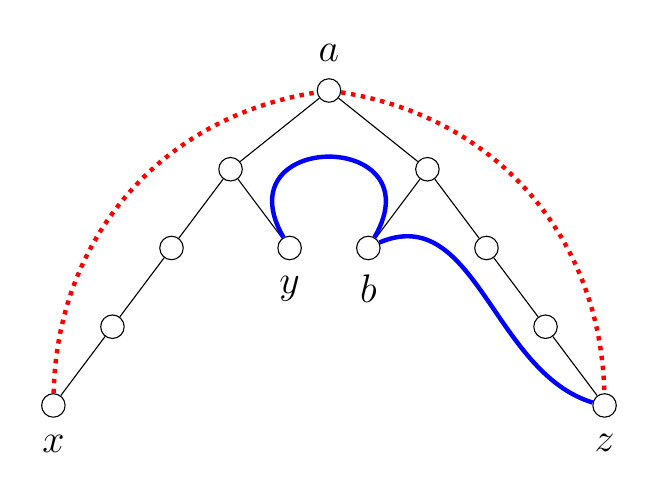
\begin{tikzpicture}[level distance=10mm, state/.style={circle, draw, minimum size=1mm}]]
  \tikzstyle{every node}=[font=\Large, draw=black,circle,inner sep=3pt, minimum size=1mm]
  \tikzstyle{level 1}=[sibling distance=25mm, set style={{every node}+=[draw=black]}]
  \tikzstyle{level 2}=[sibling distance=15mm, set style={{every node}+=[draw=black]}]
  \tikzstyle{level 3}=[sibling distance=15mm,  set style={{every node}+=[draw=black]}]
  \tikzstyle{level 4}=[sibling distance=15mm,  set style={{every node}+=[draw=black]}]
  \tikzstyle{level 5}=[sibling distance=15mm,  set style={{every node}+=[draw=black]}]


    \node[label={$a$}] (a) {}
     child {node (1) {}
      child {node (2) {}
       child {node (3) {}
        child {node[label=below:{$x$}] (x) {}}
        child[fill=none] {edge from parent[draw=none]}
       }
       child[fill=none] {edge from parent[draw=none]
        child[fill=none] {edge from parent[draw=none]}
        child[fill=none] {edge from parent[draw=none]}
       }
      }
      child {node[label=below:{$y$}] (y) {}
       child[fill=none] {edge from parent[draw=none]
        child[fill=none] {edge from parent[draw=none]}
        child[fill=none] {edge from parent[draw=none]}
        }
       child[fill=none] {edge from parent[draw=none]
        child[fill=none] {edge from parent[draw=none]}
        child[fill=none] {edge from parent[draw=none]}
       }
      }
      }
      child {node (4) {}
       child {node[label=below:{$b$}] (b) {}
        child[fill=none] {edge from parent[draw=none]
         child[fill=none] {edge from parent[draw=none]}
         child[fill=none] {edge from parent[draw=none]}
         }
       child[fill=none] {edge from parent[draw=none]
        child[fill=none] {edge from parent[draw=none]}
        child[fill=none] {edge from parent[draw=none]}
       }
      }
       child {node (5) {}
        child[fill=none] {edge from parent[draw=none]
         child[fill=none] {edge from parent[draw=none]}
         child[fill=none] {edge from parent[draw=none]}
        }
       child {node (6) {}
        child[fill=none] {edge from parent[draw=none]}
        child {node[label=below:{$z$}] (z) {}}
        }
       }
       };

    \draw[-, dotted,ultra thick,relative,red] (x) to[out=40,in=-220] (a);

    \draw[-, dotted,ultra thick,relative,red] (a) to[out=40,in=-220] (z);

    \draw[-, solid,ultra thick,relative,blue] (y) to[out=120,in=60, looseness=3.5] (b);

    \draw[-, solid,ultra thick,relative,blue] (b) to[out=60,in=200] (z);

       
\end{tikzpicture}
}
}
\end{center}